\documentclass[tikz,border=8pt]{standalone}
\usepackage{tikz}
\usetikzlibrary{positioning,arrows.meta}

\begin{document}
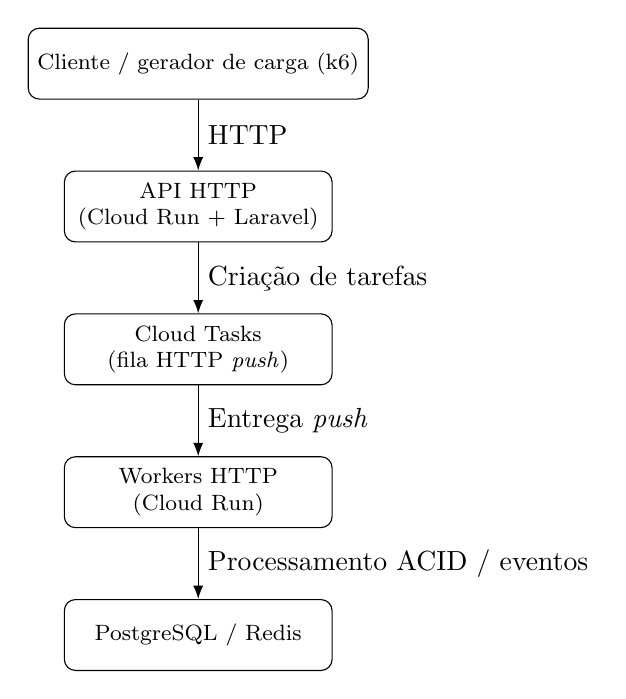
\begin{tikzpicture}[
    node distance=0.9cm,
    >=Latex,
    box/.style={
        draw,
        rounded corners,
        align=center,
        minimum width=3.4cm,
        minimum height=0.9cm,
        font=\footnotesize
    }
]
    % Coluna vertical
    \node[box] (client) {Cliente / gerador de carga (k6)};
    \node[box, below=of client] (api) {API HTTP\\(Cloud Run + Laravel)};
    \node[box, below=of api] (tasks) {Cloud Tasks\\(fila HTTP \emph{push})};
    \node[box, below=of tasks] (worker) {Workers HTTP\\(Cloud Run)};
    \node[box, below=of worker] (db) {PostgreSQL / Redis};

    % Setas
    \draw[->] (client) -- node[right]{HTTP} (api);
    \draw[->] (api) -- node[right]{Criação de tarefas} (tasks);
    \draw[->] (tasks) -- node[right]{Entrega \emph{push}} (worker);
    \draw[->] (worker) -- node[right]{Processamento ACID / eventos} (db);
\end{tikzpicture}
\end{document}
